\chapter{Probabilistic Transfer Matrix (PTM)}\label{sec:ptm}

PTM は,ゲートや回路の入力に対する出力の確率を表す行列である.
この章では,回路の信頼性を計算する既存手法として,
PTM を用いた手法について説明する.
回路全体に対応する PTM は,
基本的なゲートや結線の分岐に対応する PTM からいくつかの演算を用いて構成される.
この計算は Algebraic Decision Diagram~\redout{\cite{580054}} を用いることで,
効率的に行うことができる.

\section{ゲートや回路と対応した PTM の構築} \label{sec:ptm-const}

% 定義
$m$ 入力, $n$ 出力の部分回路を考える.
この回路に,\redout{$\bm i$ を2進数で表現した長さ $m$ のビット列 ${\it bin}(\bm i, m)$ を入力し,
出力が長さ $n$ のビット列 ${\it bin}(\bm o, n)$ となる確率を $p$ とする.}
この部分回路に対応する PTM は $2^m$ 行 $2^n$ 列で,
$M_p$ の $\bm i + 1$ 行 $\bm o + 1$ 列目の値は $p$ とする.
\[ M_p(\bm i + 1, \bm o + 1) = p \]

% 特徴
PTM の 1 行は,ある入力パターンに対して,
各出力パターンが発生する確率を表現し,その総和は 1 となる.
したがって,行列 $M$ の行と列は,それぞれ入力と出力のパターン数だけ存在する.

% 例
例えば,出力が $p = 0.05$ で反転するような AND ゲートは,
以下の様な行列で表現できる.
\begin{eqnarray}
  {\it AND}_p = \left[
    \begin{array}{cc}
      1 - p & p\\
      1 - p & p\\
      1 - p & p\\
      p     & 1 - p
    \end{array}
  \right]
= \left[
    \begin{array}{cc}
      0.95 & 0.05\\
      0.95 & 0.05\\
      0.95 & 0.05\\
      0.05 & 0.95
    \end{array}
  \right]
\end{eqnarray}
この例の 1 行目は,入力が ${\it bin}({\bm i}) = (00)_2$ となる時,出力は 0.95 の確率で ${\it bin}({\bm o}) = (0)_2$ となるが,
0.05 の確率で反転して ${\it bin}({\bm o}) = (1)_2$ となることを表している.
一方4行目は,入力が ${\it bin}({\bm i}) = (11)_2$ となる時,出力は 0.95 の確率で ${\it bin}({\bm o}) = (1)_2$ となるが,
0.05 の確率で反転して ${\it bin}({\bm o}) = (0)_2$ となることを表している.
\begin{figure}[tbp]
  \begin{center}
    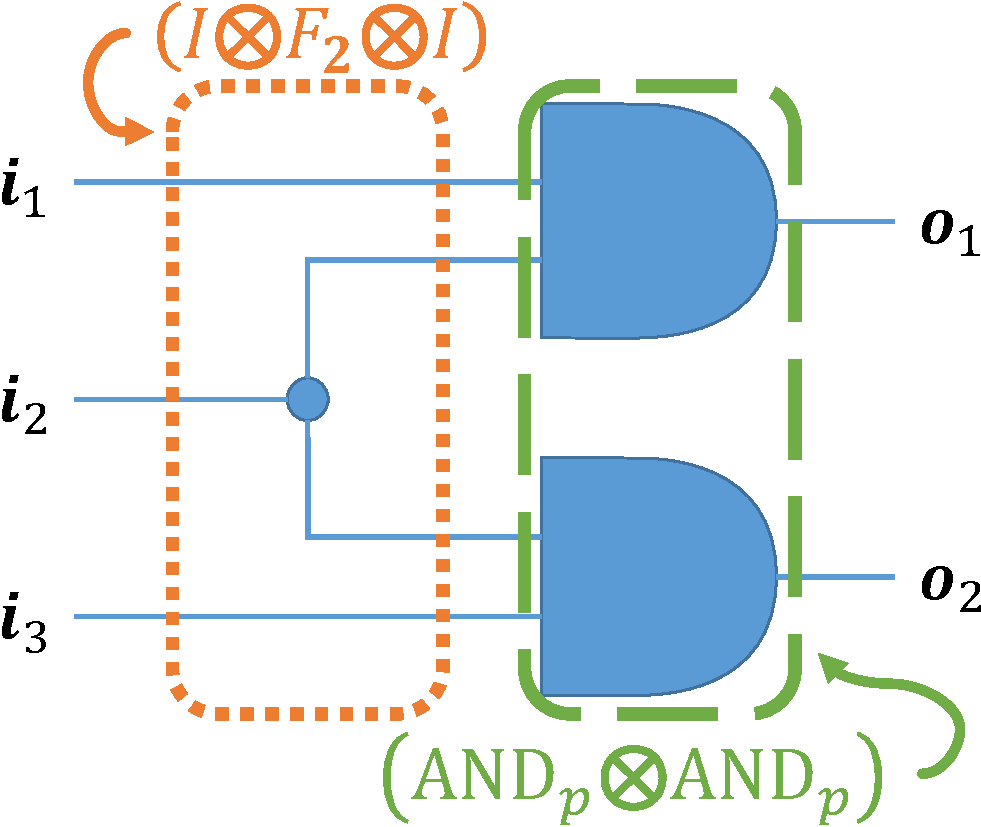
\includegraphics[height=60mm,clip]{img/exgate.pdf}
    \caption{組み合わせ回路の例}
    \label{fig:exgate}
  \end{center}
\end{figure}
また,図~\ref{fig:exgate} の回路に存在するような 2 個に分岐する部分は以下のように表す.
\[
F_2 = \left[
    \begin{array}{cccc}
      1 & 0 & 0 & 0\\
      0 & 0 & 0 & 1
    \end{array}
  \right]
\]


ゲートの直列接続に対応する PTM は,対応する PTM 同士の積に対応する.
一方,並行したゲートに対応する PTM は,対応する PTM 同士のテンソル積(クロネッカー積,$\otimes$)に対応する.
これらの計算を組み合わせることで,目的とする回路の PTM を得ることができる.

例えば,確率 $0.05$ で反転する AND ゲートを用いて図~\ref{fig:exgate} の回路を構成した時,
この回路に対応する PTM は式~(\ref{eq:ex-ptm}) のように求められる.
\begin{eqnarray}
  M_p &=& (I \otimes F_2 \otimes I)({\it AND}_p \otimes {\it AND}_p) \label{eq:ex-ptm} \\
    &=& \left(
    \left[
    \begin{array}{cccc}
      1 & 0\\
      0 & 1\\
    \end{array}
    \right]
    \otimes
    \left[
    \begin{array}{cccc}
      1 & 0 & 0 & 0\\
      0 & 0 & 0 & 1
    \end{array}
    \right]
    \otimes
    \left[
    \begin{array}{cccc}
      1 & 0\\
      0 & 1\\
    \end{array}
    \right]
    \right)
    \left(
    \left[
    \begin{array}{cc}
      0.95 & 0.05\\
      0.95 & 0.05\\
      0.95 & 0.05\\
      0.05 & 0.95
    \end{array}
    \right]
    \otimes
    \left[
    \begin{array}{cc}
      0.95 & 0.05\\
      0.95 & 0.05\\
      0.95 & 0.05\\
      0.05 & 0.95
    \end{array}
    \right]
    \right) \nonumber \\
  &=& \left[\begin{array}{cccc}
    0.9025 & 0.0475 & 0.0475 & 0.0025\\
    0.9025 & 0.0475 & 0.0475 & 0.0025\\
    0.9025 & 0.0475 & 0.0475 & 0.0025\\
    0.0475 & 0.9025 & 0.0025 & 0.0475\\
    0.9025 & 0.0475 & 0.0475 & 0.0025\\
    0.9025 & 0.0475 & 0.0475 & 0.0025\\
    0.0475 & 0.0025 & 0.9025 & 0.0475\\
    0.0025 & 0.0475 & 0.0475 & 0.9025
  \end{array} \right] \nonumber
\end{eqnarray}
最終的に得られた 8 行 4 列の行列から,各入力に対する出力の発生確率がわかる.
\redout{例えば,} $M_p(4, 2) = 0.9025$ からは,
$\bm i = 4 - 1 = (011)_2$: $i_1 = 0, i_2 = 1, i_3 = 1$ を入力した時,
0.9025 の確率で $\bm o = 2 - 1 = (01)_2$: $o_1 = 0, o_2 = 1$ が出力されることがわかる.

回路に故障が発生しない理想的な状況に対して PTM を計算すると,確率 $p$ は 0 もしくは 1 となる.
このような PTM を,特に Ideal Transfer Matrix (ITM) と呼ぶ.
図~\ref{fig:exgate} の回路に対応する ITM は,式~(\ref{eq:ex-itm}) のようになる.
\begin{eqnarray}
  M &=& (I \otimes F \otimes I)({\it AND} \otimes {\it AND}) \label{eq:ex-itm}\\
    &=& \left(
    \left[
    \begin{array}{cccc}
      1 & 0\\
      0 & 1\\
    \end{array}
    \right]
    \otimes
    \left[
    \begin{array}{cccc}
      1 & 0 & 0 & 0\\
      0 & 0 & 0 & 1
    \end{array}
    \right]
    \otimes
    \left[
    \begin{array}{cccc}
      1 & 0\\
      0 & 1\\
    \end{array}
    \right]
    \right)
    \left(
    \left[
    \begin{array}{cccc}
      1 & 0\\
      1 & 0\\
      1 & 0\\
      0 & 1\\
    \end{array}
    \right]
    \otimes
    \left[
    \begin{array}{cccc}
      1 & 0\\
      1 & 0\\
      1 & 0\\
      0 & 1\\
    \end{array}
    \right]
    \right) \nonumber \\
    &=& \left[
    \begin{array}{cccc}
      1 & 0 & 0 & 0\\
      1 & 0 & 0 & 0\\
      1 & 0 & 0 & 0\\
      0 & 1 & 0 & 0\\
      1 & 0 & 0 & 0\\
      1 & 0 & 0 & 0\\
      0 & 0 & 1 & 0\\
      0 & 0 & 0 & 1
    \end{array}
    \right] \nonumber
\end{eqnarray}

回路の最終的な信頼性は,式~(\ref{eq:fidelity}) のように,
正しい出力が得られる確率を,入力パターンが与えられる確率によって重み付き平均をとることによって評価する.
入力パターンが与えられる確率はベクトル ${\bm v}$ で表現し,${\bm i} + 1$ 番目の要素は,
${\bm i}$ を2進数としたときの入力パターンが与えられる確率を表している.
\begin{eqnarray}
  {\it fidelity}({\bm v}, M, M_p) = | {\bm v} (M_p .* M) |_{1} \label{eq:fidelity}
\end{eqnarray}
ここで, `$.*$' は要素ごとの乗算を表し, $| {\bm v} |_{1}$ は,ベクトル ${\bm v}$ の $l_1$-ノルム を表す.

%\todo[inline]{計算過程を全部書く}
図~\ref{fig:exgate} の回路に,全ての入力パターンが等確率で与えられる場合,
${\bm v}$ は,各要素は 0.125 で要素数 8 のベクトルとなる.
ここまでの例で計算した $M_p, M$ を用いて式~(\ref{eq:fidelity}) を計算すると,0.9025 という値が得られる.
\[
  M_p .* M = \left[\begin{array}{cccc}
      0.9025 & 0 & 0 & 0 \\
      0.9025 & 0 & 0 & 0 \\
      0.9025 & 0 & 0 & 0 \\
      0 & 0.9025 & 0 & 0 \\
      0.9025 & 0 & 0 & 0 \\
      0.9025 & 0 & 0 & 0 \\
      0 & 0 & 0.9025 & 0 \\
      0 & 0 & 0 & 0.9025
    \end{array}
  \right]
\]
\begin{eqnarray}
  {\it fidelity}({\bm v}, M, M_p) &=& \left|
  \left[
    \begin{array}{ccc}
      0.125 & ... & 0.125
    \end{array}
  \right] ( M_p .* M )
  \right|_{1} \nonumber \\
  &=& \left| \left[ \begin{array}{cccc}
    0.5640625 & 0.1128125 & 0.1128125 & 0.1128125
  \end{array} \right] \right|_{1} \nonumber \\
  &=& 0.9025 \nonumber
\end{eqnarray}
この結果は,ソフトエラーによって 0.05 の確率で反転する AND ゲートを用いて図~\ref{fig:exgate} の回路を構成した時,
全ての入力パターンが等確率で与えられることを仮定すると, 0.9025 の確率で正常に動作することを意味している.


\section{Algebraic Decision Diagram (ADD)を用いた計算}

% 導入
\ref{sec:ptm-const} 節の手法において,
計算の途中で発生する PTM のサイズは,指数的に大きくなる可能性がある.
与えられた 2 個の行列 $M_{1}, M_{2}$ のサイズが $k \times l$ と $m \times n$ のとき,
$M_{1} \otimes M_{2}$ のサイズは $km \times ln$ となる.
そのため,回路の中で並行した部分の入力と出力の数を $n', m'$ とすると,
$2^{n'} \times 2^{m'}$ のサイズの PTM が生成される.
この課題に対して, Algebraic Decision Diagram (ADD)
\cite{580054} を用いた手法 \cite{Krishnaswamy:2008:PTM:1297666.1297674} が提案された.
ADD は Binary Decision Diagram (BDD)~\cite{BLTJ:BLTJ1585} から派生したデータ構造で,
行列内の部分的に共通した情報を省略して保持しながら計算することができる.

% ADD の説明
ADD は,無閉路有向グラフ $(\Phi \cup V \cup T, E)$ として
$\{0, 1\}^n \mapsto S$ の関数の集合を表す.
\redout{ここで,}$S$ は定数の集合である.
$\Phi$ は入次数 0,出次数 1 の開始節点であり,その ADD で表現したい関数と 1 対 1 で対応する.
中間節点 $V$ は,関数が依存する変数を表して\redout{いるため},出次数は 2 となる.
この 2 個の辺は,1-枝と0-枝と呼ばれ\redout{る.
関数をの結果を得る際には,節点の変数に 0 を割り当てた場合は0-枝,
1 を割り当てた場合は1-枝をたどり,終端節点 $T$ を探索する.}
終端節点は,変数割り当ての結果として $S$ に含まれる定数でラベル付けされている.
BDD では論理関数を再帰的に表現し,終端節点は定数関数を表す 1 か 0 となる\redout{.
一方,}ADD では,終端節点の扱い方を変更し,0, 1 に限らない任意の終端節点を持つことができる.

\begin{figure}[tb]
  \centering
  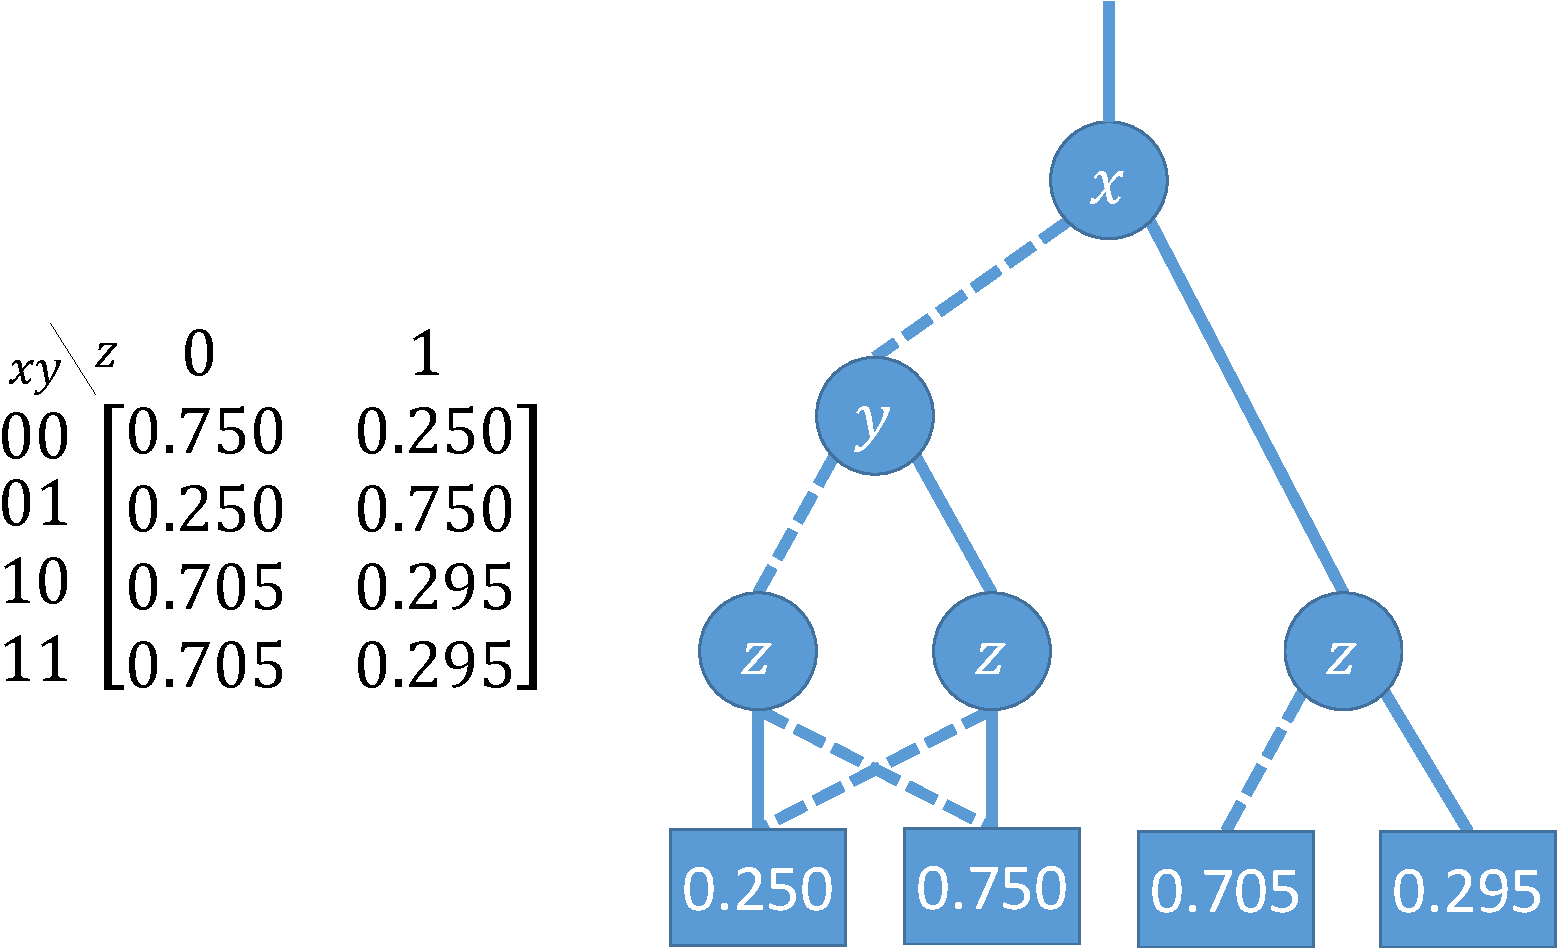
\includegraphics[height=70mm]{img/add-sample}
%  \missingfigure[figwidth=60mm]{ADD の画像を入れる}
  \caption{ADD によって行列を表現する例}
  \label{fig:ex-add}
\end{figure}
行列を ADD で表現した際のグラフ構造の例を図~\ref{fig:ex-add}に示す.
1-枝と0-枝は,それぞれ実線\redout{の}矢印と破線\redout{の}矢印で表されている.
各節点で場合分けを行う決定変数が 1 の場合は1-枝,0の場合は0-枝に対応し,
根節点から終端節点への 1 本のパスは, $\{0, 1\}^n$ と定数の対応を表している.
すなわち,各非終端節点は決定変数でラベル付けされて\redout{いるため},
決定変数の割り当て通りに\redout{枝を}たどることで,対応する定数を得ることができる.

\begin{figure*}[tb]
  \begin{minipage}{0.5\hsize}
    \centering
    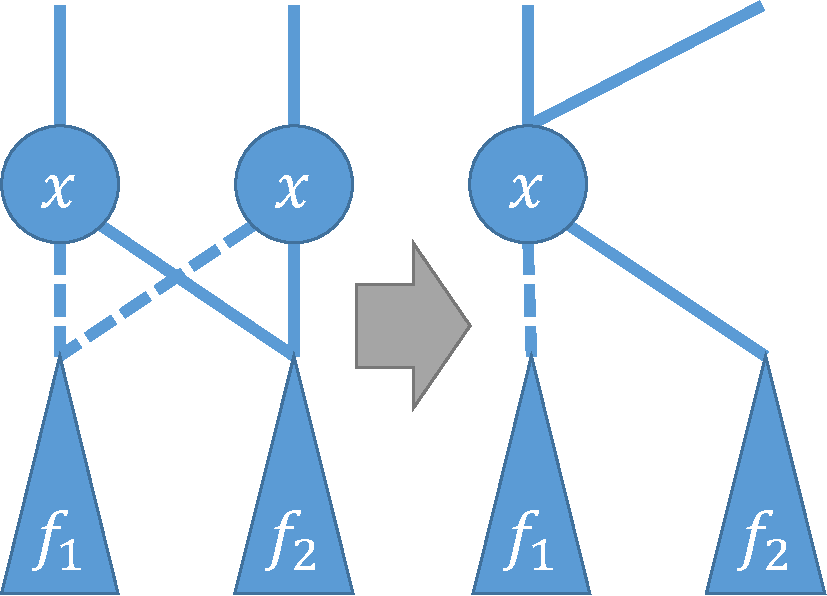
\includegraphics[height=50mm]{img/add-share-rule.pdf}
%    \missingfigure[figwidth=60mm]{サブグラフのマージ}
    \caption{等価な節点の共有}
    \label{fig:add-marge}
  \end{minipage}
  \begin{minipage}{0.5\hsize}
    \centering
    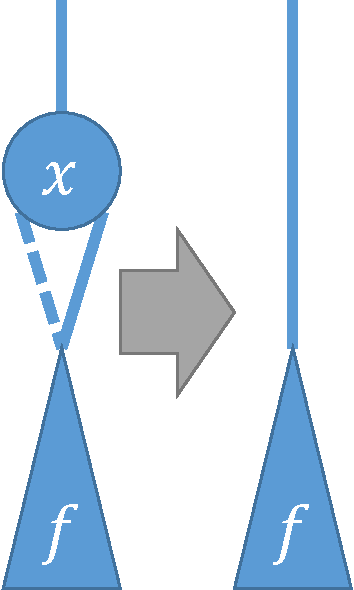
\includegraphics[height=50mm]{img/add-needlessly-rule.pdf}
%    \missingfigure[figwidth=60mm]{冗長な節点の削除}
    \caption{冗長な節点の削除}
    \label{fig:add-remove}
  \end{minipage}
\end{figure*}
ADD は変数の順序を固定し,等価な節点の共有と冗長な節点を削除することによって,
コンパクトかつ一意な表現を得ることができる.
2つの節点 $v_i, v_j$ が以下を満すとき,この2つの節点は等価であり,
図~\ref{fig:add-marge} のように共有することができる.
\begin{itemize}
  \item $v_i$ と $v_j$ \redout{にラベル付けされた決定変数が同じ}
  \item $v_i$ と $v_j$ の0-枝が同じ節点を指す
  \item $v_i$ と $v_j$ の1-枝が同じ節点を指す
\end{itemize}
$v_i, v_j$ が終端節点の場合には,ラベル付けされた定数のみを比較して等価性を判断する.
また,ある節点の0-枝と1-枝が同じ節点を指すとき,この節点は冗長なので,
図~\ref{fig:add-remove} のように削除することができる.
図中の $f_1, f_2, f$ は ADD の部分グラフである.

また,2 個の ADD を入力し,それらの二項演算の結果を直接生成するアルゴリズムが考案されている.
これらのアルゴリズムは,
一意性についてのキャッシュテーブルと演算についてのキャッシュテーブルを利用することで効率的に計算することができる.
ADD を用いて PTM を計算する手法では,必要な演算を追加で定義し,同様の効率性を持ったまま計算することができる.

%\chapter{Zero-suppressed Binary Decision Diagram}
%\todo[inline]{TODO: ZDD の数式処理がうまくいったら入れる}
